%%%%%%%%%%%%%%%%%%%%%%%%%%%%%%%%%%%%%%%%%%%%%%%%%%%%%%%%%%%%%%%%%%%%%%%%%%%%%%%%

\documentclass[12pt, a4paper, oneside]{article}

\input{/home/giatro/.config/user/giatro_packages.tex}

\input{/home/giatro/.config/user/giatro_macros.tex}

\title{Lista 2 - MAC0425 - Inteligência Artificial}
\date{\today}
\author{Lucas Paiolla Forastiere - 11221911}

%%%%%%%%%%%%%%%%%%%%%%%%%%%%%%%%%%%%%%%%%%%%%%%%%%%%%%%%%%%%%%%%%%%%%%%%%%%%%%%%
%%%%%%%%%%%%%%%%%%%%%%%%%%%%%%%%%%%%%%%%%%%%%%%%%%%%%%%%%%%%%%%%%%%%%%%%%%%%%%%%

\begin{document}

\maketitle

\paragraph{1.}%
\label{par:1_}

Os experimentos foram feitos utilizando os arquivos \texttt{qlearn.py} e
\texttt{explore-qlearn.py} (basta ter \texttt{python} e a biblioteca
\texttt{numpy} instalados e rodar utilizando \texttt{\$ python qlearn.py} ou
\texttt{\$ python explore-qlearn.py}).

O programa que se chama apenas \texttt{qlearn.py} obtém os q-valores sem fazer
nenhuma exploração. Apenas aplicamos a fórmula do algoritmo em cada entrada da
matriz $3\times 4$ várias vezes até convergir. Após 5 iterações, temos os
seguintes q-valores:

\begin{figure}[h]
\centering
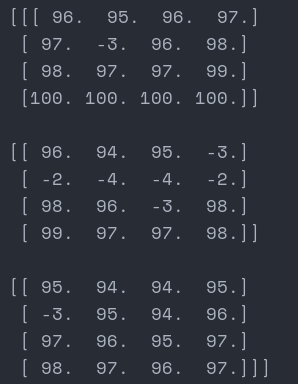
\includegraphics[scale=0.8]{Res/q-values-ex1.png}
\caption{O \texttt{ndarrary} dos \textit{q-values} para o exercício 1. Como cada
estado possui 4 ações, então temos um tensor de três dimensões. Cada bloco de 4
arrays se refere a uma linha do mapa. Observe como a quarta linha são apenas
valores $100$. Isso é devido ao fato de esse ser o nosso estado final que tem
recompensa $100$.  Cada um dos valores de uma linha representa o q-valor de ir
naquela direção. Na ordem temos: esquerda, cima, direita e para baixo. Portanto,
se quisermos saber o q-valor de ir para a esquerda na posição $2,3$ da matriz,
basta olhar o segundo conjunto de $4$ linhas, dai a terceira linha desse
conjunto e olhar o primeiro valor dessa linha. Vemos que é $-3$, o que faz
sentido, pois a casa da esquerda leva a uma recompensa negativa.}
\label{q-values-ex1.png}
\end{figure}

Para facilitar a visualização, eu também coloquei para mostrar um mapa
esquemático de como está a política referente aos q-valores exibidos.

\begin{figure}[h]
\centering
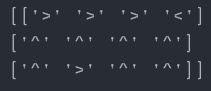
\includegraphics[scale=0.9]{Res/policy-ex1.png}
\caption{A política referente à figura anterior.}
\label{policy-ex1.png}
\end{figure}

O programa \texttt{explore-qlearn.py}, por sua vez, considera que temos um
agente explorando esse mapa e que realiza um episódio por vez, começando no
estado final e terminando quando chega ao estado final. Para fazer essa
exploração, nós adotamos a estratégia chamada de \textit{epsilon-greedy}, que
sempre segue a atual política ótima a menos de uma chance $\epsilon$ de fazer
uma ação completamente randômica (adotei $\epsilon=0.3$).

Além disso, foi levado em conta que o agente, após escolher uma ação, tem apenas
$80\%$ de chances de realmente conseguir fazer aquela ação e $10\%$ de acabar
indo para um dos lados adjacentes, como proposto em aula pelo professor. Quando
o agente acaba indo para um lugar que ele não queria ir, ele não sabe disso. A
única informação que ele recebe é a recompensa pela ação que ele pensa que tomou
e, portanto, o q-valor que vamos atualizar é aquele referente a ação que o
agente \textit{acha} que tomou, não de fato a que ele acabou fazendo sem querer
(indo parar em um lugar que não pretendia).

É interessante que, mesmo com essa mecânica, os q-valores convergem exatamente
para os mesmos que anteriormente na figura \ref{q-values-ex1.png}, assim como a
política ótima, evidentemente.

O número de episódios que precisamos para chegar nesse resultado, entretanto, é
relativamente alto, cerca de $45$ (como o comportamento do agente é
não-determinístico, esse valor varia).

\paragraph{2.}%
\label{par:2_}

Para o segundo exercício, temos que o estado $3,4$ tem uma recompensa de $+10$.
Isso faz com que nossos dois algoritmos anteriores não convirgam para valor
nenhum. O primeiro algoritmo (\texttt{qlearn.py}, que não explora) vai
aumentando os q-valores a cada iteração, ficando todos eventualmente infinitos.
Já no que exploramos, isso acontece também, mas as ações que levam ao estado de
recompensa negativa ainda possuem q-valores negativos.

Na prática, quando rodamos o algoritmo em que há um agente explorando, cada
epsódio dele vai ficando mais e mais demorado, pois ele tenta passar o máximo de
vezes que ele consegue pelo estado de recompensa $10$ antes de terminar o
epsódio.

A pergunta feita na lista é se isso corresponde ao esperado. Minha resposta é
que sim, pois esse é de fato o comportamento que \textit{se espera} caso nós não
colocamos nenhuma punição no agente por ficar andando muito tempo antes de
terminar um epsódio. Todavia, esse não é o comportamento \textit{desejado}.
Desejamos uma trajetória em que o agente passa pelo $10$ uma única vez e vai
direto para o estado final.

Para isso, precisamos modificar o valor de $\gamma$, que é o coeficiente de
penalização do agente por levar muitos passos para finalizar um epsódio. Nos
casos anteriores, $\gamma$ era igual a $1$.

Tomando um valor de $\gamma$ muito pequeno, como $0.5$, temos que o agente quer
terminar o epsódio tão rápido, que ele nem passa pelo $10$, levando aos
q-valores da figura \ref{q-values-ex2.1.png} e política da figura
\ref{policy-ex2.1.png}.

\begin{figure}[h]
\centering
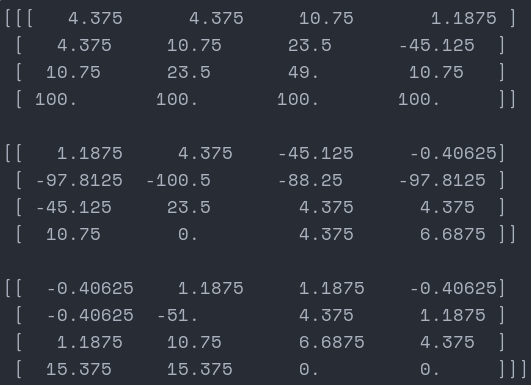
\includegraphics[scale=0.7]{Res/q-values-ex2.1.png}
\caption{Q-valores para o exercício $2$ com $\gamma=0.5$.}
\label{q-values-ex2.1.png}
\end{figure}

\begin{figure}[h]
\centering
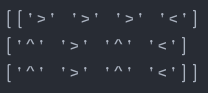
\includegraphics[scale=0.9]{Res/policy-ex2.1.png}
\caption{Política para o exercício $2$ com $\gamma=0.5$. Vemos que o agente
sequer passa pela casa $3,4$, que é onde temos uma recompensa de $+10$, pois o
desconto por andar mais é tão grande que não vale a pena.}
\label{policy-ex2.1.png}
\end{figure}

Por outro lado, se colocamos um valor não tão grande de penalidade, como
$\gamma=0.9$, temos os resultados das figuras \ref{q-values-ex2.2.png} e
\ref{policy-ex2.2.png}.

\begin{figure}[h]
\centering
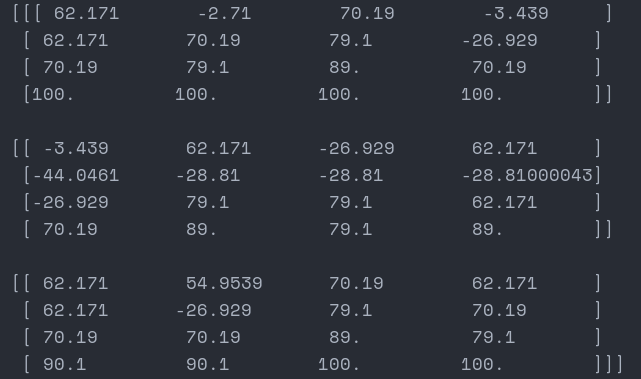
\includegraphics[scale=0.8]{Res/q-values-ex2.2.png}
\caption{Q-valores para o exercício $2$ com $\gamma=0.9$.}
\label{q-values-ex2.2.png}
\end{figure}

\begin{figure}[h]
\centering
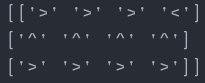
\includegraphics[scale=0.8]{Res/policy-ex2.2.png}
\caption{Política para o exercício $2$ com $\gamma=0.9$. Vemos que agora o
agente escolhe ir para a direita sempre que possível na última linha, pegando a
recompensa de $+10$ e se está na posição $3,4$, ele também escolhe ir para a
direita, permanecendo no lugar e ganhando uma recomepensa de $+10$ novamente. E
caso ele acabe indo para cima sem querer, então ele termina seu epsódio.}
\label{policy-ex2.2.png}
\end{figure}

Portanto, vimos que para fazer o agente ter o resultado que gostaríamos, basta
modificar o valor de $\gamma$ de forma a punir mais ou menos ele por ficar
andando demais.

Para convergir, tomamos muito mais tempo agora, cerca de $80$ episódios.




%%%%%%%%%%%%%%%%%%%%%%%%%%%%%%%%%%%%%%%%%%%%%%%%%%%%%%%%%%%%%%%%%%%%%%%%%%%%%%%%

\end{document}
